\documentclass[main.tex]{subfiles}

\begin{document}
\pagebreak

\section{A2 Git: Konflikte bereinigen}
Nutzen  Sie weiterhin Ihr erstelltes Repository aus Aufgabe A1.

\lstset{language=bash}

\lstset{style=MyCodeStyle}

\renewcommand{\labelenumi}{\arabic{enumi}.}

\begin{enumerate}
\item Für diesen Aufgabenteil müssen zwei entwickelnde Personen an verschiedenen Rechnern mit eigenen Klonen des Repository arbeiten. Alternativ können Sie auch an einem Rechner einen zweiten Klon des Repository in einem anderen Verzeichnis erzeugen und über
\lstinline|git config --local|
einen anderen Benutzernamen und eine andere Mailadresse wählen. Die verschiedenen Namen der Entwickler sind für den Commit-Verlauf wichtig.
\item Stellen Sie zunächst sicher, dass beide Repositories auf dem aktuellen Stand sind.
\item Erzeugen Sie nun in einer bestehenden Quellcodedatei einen Konflikt in einer Codezeile,
z.B. indem Sie im ersten Repository „Hello World!“ durch einen Parameter und im zweiten Repository durch einen String in einer anderen Sprache ersetzen.

\item Versuchen Sie nun, beide Änderungen in das Remote-Repository zu übertragen. Bei einem Repository wird es gelingen, beim anderen wird es mit einer Fehlermeldung scheitern.
\item Beheben Sie den Konflikt in dem Repository, bei dem das Übertragen gescheitert ist, indem Sie beide Änderungen geeignet kombinieren.
\item Übertragen Sie dann die neue, konfliktfreie Version zurück ins Remote-Repository.
\item Prüfen Sie den Commit-Verlauf mit \lstinline|git log --graph|.

\end{enumerate}

\subsection{Lösung 2}

\begin{figure}[H]
    \makebox[\textwidth][c]{
        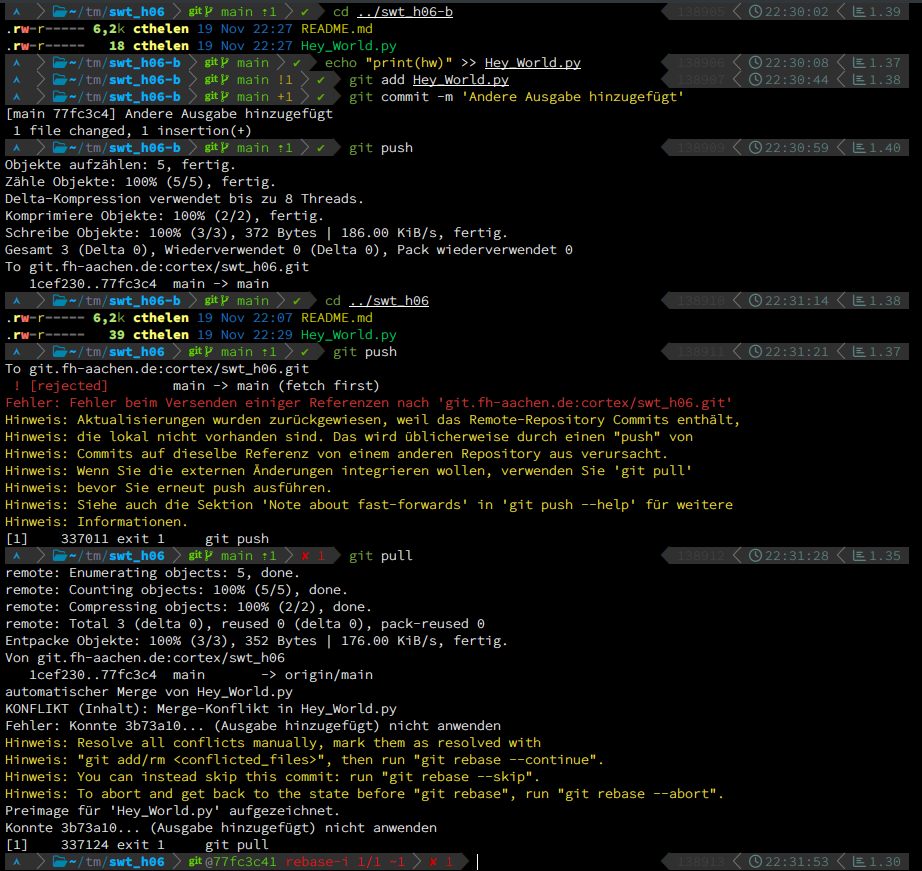
\includegraphics[width=1.2\linewidth]{s4.png}
    }
    \caption{Aufgabe 2, Nr. 1-4}
    \label{fig:a1}
\end{figure}
\begin{figure}[H]
    \makebox[\textwidth][c]{
        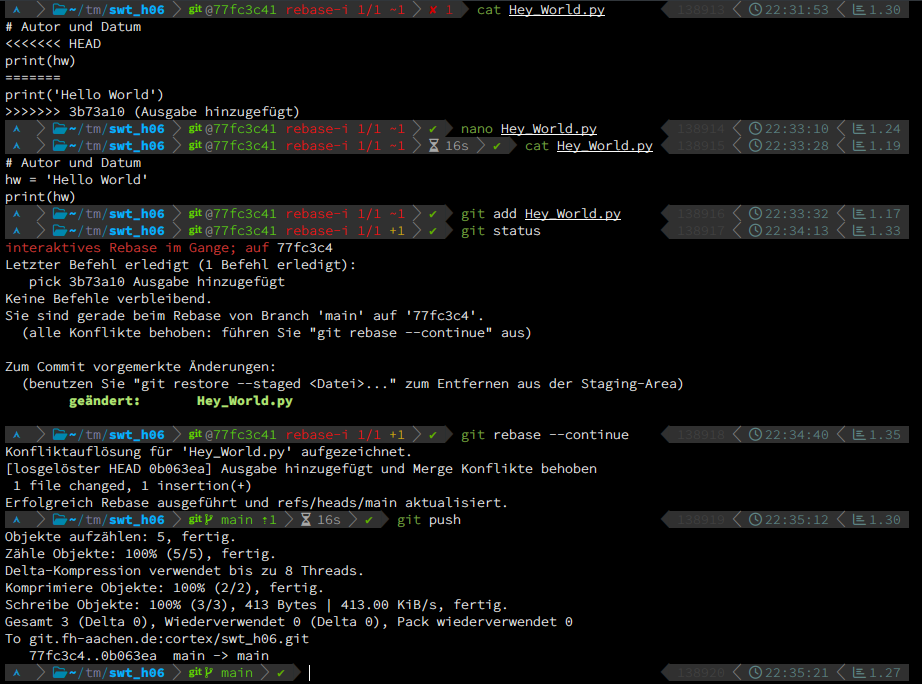
\includegraphics[width=1.2\linewidth]{s5.png}
    }
    \caption{Aufgabe 2, Nr. 5-6}
    \label{fig:a1}
\end{figure}
\begin{figure}[H]
    \makebox[\textwidth][c]{
        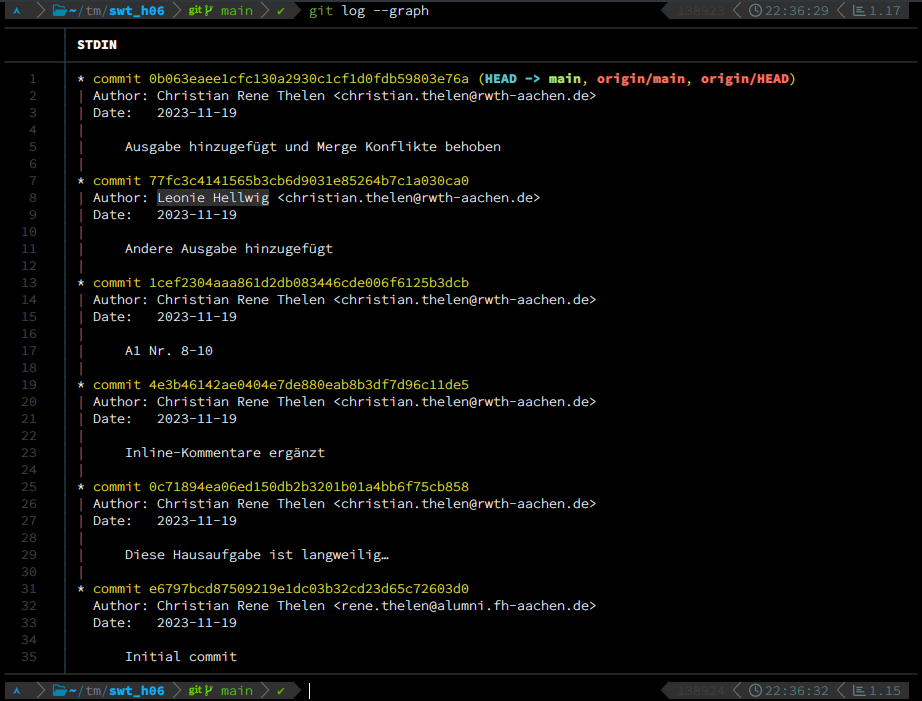
\includegraphics[width=1.2\linewidth]{s6.png}
    }
    \caption{Aufgabe 2, Nr. 7}
    \label{fig:a1}
\end{figure}

\end{document}
